\documentclass[a4paper]{article}

\usepackage[english]{babel}
\usepackage[utf8x]{inputenc}
\usepackage[T1]{fontenc}

\usepackage[a4paper,top=3cm,bottom=2cm,left=3cm,right=3cm,marginparwidth=1.75cm]{geometry}

\usepackage{nth}
\usepackage{amsmath}
\usepackage{graphicx}
\usepackage[hidelinks]{hyperref}
\usepackage{enumitem}

\newcommand{\ts}{\textsuperscript}

\title{Integrated Group Project}
\author{NA3
	\\ \rule{5cm}{0.4pt}
	\\Charlie Howes, Lewis Allen, 
    \\Adam Howes, Ben Ashing, 
    \\Constantinous Ioannou
    \\ \rule{5cm}{0.4pt}
} %TODO: Look at making the rule closer to the text.

\begin{document}
\maketitle

\tableofcontents

\pagebreak

\section{Planning}
\subsection{Gantt Chart}
\subsubsection{Proposed}
\subsubsection{Actual} %TODO: This might be better at the end, but not 100% sure.

\subsection{Minutes}

\pagebreak

\section{Requirements}

\subsection{Document} %TODO: Need to rename one of these.

\begin{enumerate}
  \item Business Requirements
  \begin{enumerate}[label=B\arabic*.]
    \item The Planning should be completed by March \nth{13}
    \item The finished product should be delivered in May.
    \item The software will be adopted and used by all staff.
  \end{enumerate}

  \item User Requirements
  \begin{enumerate}[label=U\arabic*.] 
    \item Users must be able to log in using a user name and password.
    \item Users must be able to log out
    \item The user must be able to personalize their view.
    \item The user must able to easily view calendars for daily, monthly and yearly schedules.
    \item The user must be able to set recurring appointments.
    \item Staff must be able to create groups.
    \item Staff must be able to modify groups
    \item Staff must be able to add other staff/groups to events.
    \item The user must be able to cancel appointments at any time within a session.
    \item The user must be able to use a search feature to find other users.
    \item The user should be able to make event requests. 
    \begin{enumerate}[label*=\arabic*.]
      \item Users should be able to accept event requests.
      \item Users should be able to decline event requests
    \end{enumerate}
    \item Receive invitations  %Indent - as this is to do with event requests
    \item The User should be able to accept or decline events. %Indent this by one?
  \end{enumerate}

  \item Quality Requirements
  \begin{enumerate}[label=Q\arabic*.]
    \item The application must use symbols to clearly show changes in events.
    \item The application should notify the user in any changes to events such as cancellations.
    \item The application must implement optimized loading times.
  \end{enumerate}
  \item Functional Requirements
  \begin{enumerate}[label=F\arabic*.]
    \item Only members of staff should be assigned accounts.
    \item The architecture of the project should support different platforms.
    \item A method must exist which allows staff to be given administration rights to form an administrative team.
    \item Administrators must be able to verify accounts.
  \end{enumerate}
  \item Non-Functional Requirements
  \begin{enumerate}[label=NF\arabic*.] %TODO: These need to be completed fully. More added?
  	  \item The user should be able to complete any single task with a minimum of eight actions (LA)
      \item The code needs to be easily maintainable by keeping the code organized, well written, documented and simple. (CH)
      \item The project must be easily scaled to implement new features and a larger user base. (CH) %TODO: Be more specific with numbers
      \item The product must be executable on all standard desktop Operating Systems with X minimum specifications. (AH)
      \item All personal data must be fully secure through encryption and hashing. (BA)
      \item The project must be adaptable in the future for mobile implementations. (CI)
  \end{enumerate}
\end{enumerate}

\clearpage % Forces the figure to be in this subsection by clearing the floats.
\subsection{Stakeholder Diagram}

\begin{figure}[!ht]
    \centering
    \makebox[0.75\textwidth]{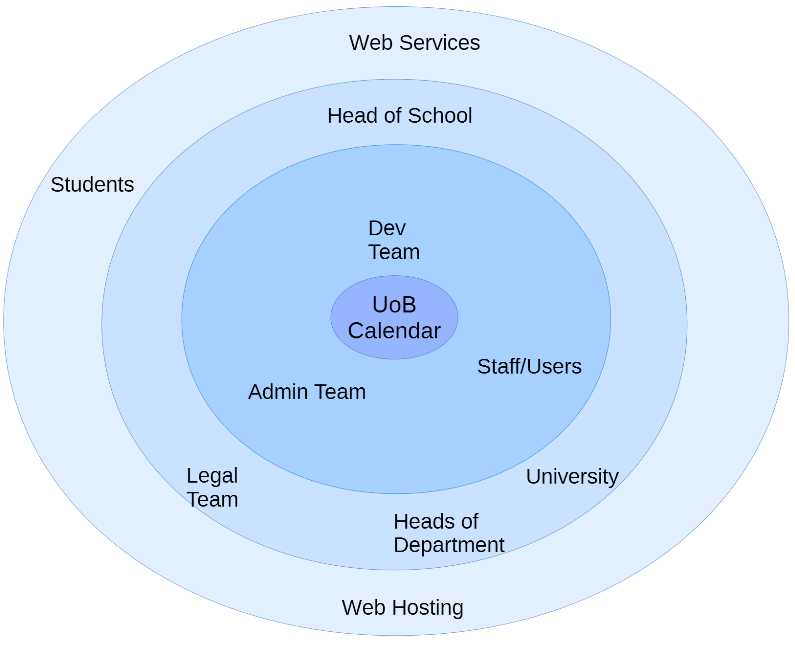
\includegraphics[width=0.75\paperwidth]{OnionModel.png}} %TODO: Check this sizing at the end.
    \caption{Stakeholder Diagram}
    \label{fig:stakeholder}
\end{figure}

\section{Use Case Model}

\subsection{Actors}

\subsection{Diagram}

\subsection{Case Descriptions}

\section{Class Diagram}

\section{Database}
\section{Entity Relationship Diagram}

\section{Design}

\end{document}